\paragraph{La classe Thesaurus}

\begin{minipage}
    {\linewidth}
    \centering
    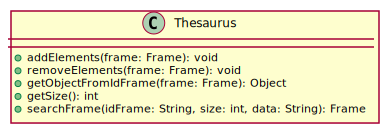
\includegraphics[width=0.80\linewidth]{../schemas/Conception_detaillee/classe_thesaurus.pdf}
    \captionof{figure}{Diagramme de classe de Thesaurus}
\end{minipage}

\subparagraph{Philosophie de conception \newline} 

\medspace

La classe Thesaurus a pour rôle de répertorier sous la forme d'un dictionnaire les trames qui sont envoyées par l'application {\nomApplication}.

\subparagraph{Description structurelle \newline}

\medspace

\textbf{Attributs :}

N.A.

\textbf{Services offerts :}

\begin{itemize}
    \item \textbf{getObjectFromIdFrame(idFrame : String) : Object} --- Opération qui recherche dans le dictionnaire la trame correspondant à l'identifiant "idFrame". Cet identifiant est lié à un objet qui est retourné afin de savoir si un objet contient cette trame.
    \item \textbf{addElements(frame: Frame): void} --- Opération qui permet d'ajouter un élément au dictionnaire.
    \item \textbf{removeElements(frame: Frame): void} --- Opération qui permet de supprimer un élément du dictionnaire. 
    \item \textbf{getObjectFromIdFrame(frame: Frame): Object} --- Opération qui permet de récupérer l'objet à partir d'une trame.
    \item \textbf{getSize(): int} --- Opération qui permet de retourner la taille du dictionnaire. 
    \item \textbf{searchFrame(idFrame: String, size: int, data: String): Frame} --- Opération qui permet de trouver la trame correspondante dans le dictionnaire sans posséder tous les attributs. 
\end{itemize}